\documentclass[11pt]{article}

\usepackage{cite}
\usepackage{graphicx}
\graphicspath{{img/}}
\usepackage{hyperref}
\usepackage[linesnumbered,lined,boxed,commentsnumbered]{algorithm2e}



\begin{document}

% Subject : Symbolic executions technique for finding bugs %
\title{A Survey of\\Symbolic Executions Techniques} % NB: I removed the "for finding bugs" because "bug" is not well-defined and we can clearly state in the introduction why we use symbolic execution.
\author{Hallet Adrien \and Sens Loan}
\date{\today}
\maketitle

  \section*{Abstract}
    % Describe paper's goals and content

  \section{Introduction}
    \subsection{A definition}
      % I tried to explain what is symbolic execution in simple concepts of software engineering
      The first occurences of symbolic execution described the then-new method as a middle ground~\cite{newapproach} between the two most-used method of its time. On one hand, program testing (\emph{e.g.: unit testing}) can not always detect a fault in a program and producing a correct test sample and proving that it indeed is correct is not that easy. On the other hand, program proving can indeed ensure that a program is correct from its entry point to the result but it heavily relys on the proof definitions by the programmer and the formal definition of the problem.\\
      Nowadays, symbolic execution is both described as (part of) the core of many modern techniques to software testing\cite{chopper:icse18} and an effective way to create tests suites with extensive coverage.\cite{threedecadeslater}
    \subsection{The concept}
      The idea behind symbolic execution is to test an algorithm with \emph{symbolic values} rather than concrete values. So instead of using unit testing where a variable is set to a (usually random) value, the symbolic execution maintains a formula that contains all the possible values for the code to reach a particular point in the program. This formula is updated every time the program reaches a branching point. In figure~\ref{fig:symbolicsimple}, we show an example from~\cite{visserWillemCorina} of a symbolic execution. Notice how it produces constraints over the variables to explore the algorithm's branching tree.
      \begin{figure}
        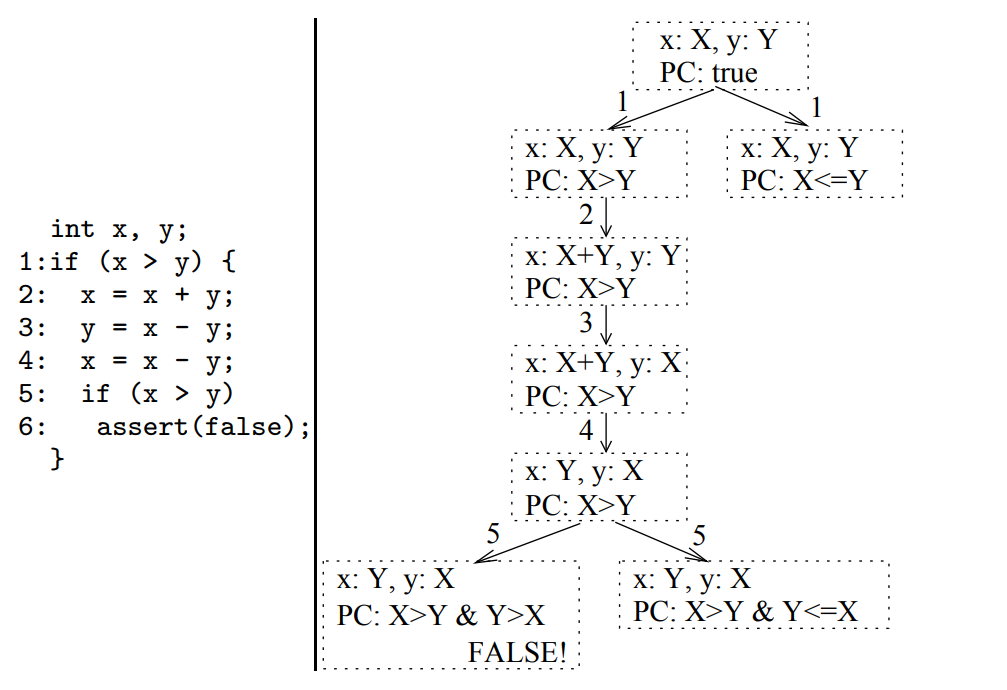
\includegraphics[width=0.5\textwidth]{symbolicsimple}
        \caption{Swapping two integers and its symbolic execution tree}
        \label{fig:symbolicsimple}
      \end{figure}
    % What is symbolic execution and why do we do this survey

  \section{History}
    % Draft the history of symbolic execution, dig any trend up or whatever we can say about it.

  \section{Method}
    % Begin with anything general to say (if any) then detail methods, could also be useful to compare them (if possible) and/or to say when/why a particular method is being used instead of another.
    \subsection{Useful concepts}
      Algorithms can be modeled as graphs where nodes are basic blocks (\emph{i.e.: a part, one or multiple instructions with a single entry and exit point}) and edges are the branches (issued from conditional statements). Def-use pairs use the same concept, although they base their graph on the \emph{definition} and \emph{usage} of a variable. With the \emph{branches} and \emph{def-use pairs}, we can model an algorithm's behavior to follow the values of its variables and determine the \emph{execution path}.
    \subsection{Basis}
      \label{sub:basis}
      Symbolic execution works on those concepts by updating an internal list of symbols. The execution generates a new symbol for each introduced variable in an algorithm\cite{newapproach}. The symbolic execution runs over the algorithm's statements and builds the symbolic values when it encounters a branching point. The symbolically executed algorithm creates a \emph{state}\cite{visserWillemCorina} containing the symbolics values, a counter identifying the next line to be executed and a \emph{path condition}. This path condition is a simple boolean formula over the symbols, it creates a constraint for the algorithm to reach the current state of the program (this also allows to check for unreachable paths in programs~\cite{InfeasiblePathsEliminationWithSymbolicExecTechniques}). The path condition allows to recreate the execution up to its state. The states are stored in a \emph{symbolic execution tree} with the states as nodes and the transitions as edges (see figure~\ref{fig:symbolicsimple}).
    \subsection{Problems}
      Symbolic Execution cannot be that perfect and hosts its bundle of problems that reduce either the confidence in or the performances of the concept. We have seen symbolic execution tree in~\ref{sub:basis}. Small algorithms can use such methods but actual programs need to be tested in \emph{integration}. In large environments, the tree's branching factor will produce too many nodes (\emph{state-space explosion}) for the performances to stay relevant, sometimes creating infinite loops in the graph~\cite{forwardSymbolicExecution}. Reducing the state space or pruning them is not enough. To improve the performances, we can depth-first-search the graph but it does not prevent infinite loops until we add a max depth (as KLEE or EXE do). %TODO: Ref the tools when (if) we cite them.
      Pruning heuristics (\emph{e.g.:def-use pairs distance}) can be used to reduce the tree's branching factor, we may randomly select a path (emph{i.e: the path condition}), weighting the shallowest nodes to avoid dead-loops. The random technique is exploited by a lot of \emph{fuzzing techniques}~\cite{CHEN2018118} which uses the injection of random values to detect program's faults. Another solution lies in the \emph{concolic execution} (see~\ref{subsec:concolicExecution}).
      %TODO: Adrien => explore the in-memory variable problem and see if there are others.
  \section{Variants}
    % I split the section because it was too heavy for my liking and I think we can better state the base and what challenges it produces, then look at how we can solve them with variants. It also allows the reader to just skip the variants in the future if he just wants to know about the method.
    \subsection{Concolic execution}
    \label{subsec:concolicExecution}
    	The name "concolic" is a portmanteau of the words "concrete" and "symbolic", the idea of this testing method is to mix symbolic execution alongside concrete ones.\\

    	\begin{figure}
    		\centering
    		
\includegraphics[width=0.34\columnwidth]{concrete-abstract.eps}
			\caption{Concrete and abstract execution machine models}
			\label{fig:concrete-symbolic}
    	\end{figure}

    	\subsubsection*{Concolic execution approaches}
    		This technique concept was first introduced on 2005 \cite{godefroid2005dart} (more details on section \ref{subsec:DART}). % The name used wasn't "Concolic" yet but the concept idea was the same
    	Since then the idea was further extended and combined with other testing techniques.\\

    	However, the general principle has been explored with different angles.

    		\subsubsection{Dynamic Symbolic Execution}
    		\label{subsec:dynamicSymbolicExec}
    			\emph{Dynamic Symbolic Execution} (DSE) also kwown as \emph{dynamic test generation} \cite{godefroid2005dart} is a popular approach of concolic execution. Its main feature is to have the concrete execution drive the symbolic execution.\\

    			This method need to add a new store in order to save the concrete execution information.\\
    			We first choose an arbitrary value as input for our parameters. Then it executes the program concretely and symbolically at the same time updating both stores and the path constraints. Whenever the concrete execution takes a branch, the symbolic execution is directed toward the same branch and the constraints extracted from the branch condition are added to the current set of path constraints.\\
    			In order to explore different paths, the path conditions given by one or more branches can be negated and the solver invoked to find a satisfying assignment for the new constraints.\\
    			We can repeat this process as many time as we want to achieve the desired coverage.\\
    			
    			Notice that it exists different strategies on the choice of the branch to negate, this crucial heuristic choice depends of the tool.\\
    		
    		\subsubsection*{Downside : Imperfect symbolic execution}
    			\begin{description}
    				\item[False Negative] Missed path. For example, when another function from the one tested is not symbolically tracked but its result is needed to explore a particular path.
    				\item[Path Divergence] In some situations the engine can't guess that no input can provoke an error. In other word, whenever an actual execution path does not match the program path predicted by symbolic execution for a given input vector. For example, assert on a negative value of an absolute value due to the untracked side effect of the \texttt{abs()} function.\\
    				According to \cite{Godefroid2008AutomatedWF} they calculated a divergence rates of over 60 \%
    			\end{description}


  \section{Tools and languages}
  	Many tools exist for symbolic execution, \href{https://en.wikipedia.org/wiki/Symbolic_execution\#Tools}{Wikipedia} mention 22 of them. Another \href{https://github.com/ksluckow/awesome-symbolic-execution\#tools}{source} claiming to "curate a list of awesome symbolic execution resources including tools" mention 35 different tools spread over 10 different languages.\\ %TODO [Loan] : est-ce qu'on ajoute ça dans la bliblio ?
  	
    % Anything general to say bout the content (maybe explain the omnipresence of Microsoft in the market)
    % List tools and language, compare them if possible

    % Let DART be first as it is the first used tool to use concolic
    \subsection{\emph{DART} : Directed Automated Random Testing}
    \label{subsec:DART}
    	\emph{DART} is presented as a tool for automatically testing software using concolic testing method. It was introduced in 2005 making it the first the first tool to be created using concolic techniques and more specifically dynamic symbolic execution techniques (see section \ref{subsec:dynamicSymbolicExec}). \\

    	\subsubsection{Methodology}
	    	\emph{DART} combines three main techniques 	    	\cite{godefroid2005dart} in order to automate the process of testing for a particular software :
	    	\begin{enumerate}
	    		\item An automated extraction of the interface of a program with its external environment using static source-code parsing
	    		\item An automatic generation of a test driver for this interface that performs random testing to simulate the most general environment the program can operate in
	    		\item A dynamic analysis of how program behaves under random testing and automatic generation of new test inputs to direct systemically the execution along alternatives program paths
	    	\end{enumerate}
	    		    	
			\emph{DART} chooses the \emph{depth-first} strategy whenever it has to negate a branch.
	    
	    \subsubsection{Example}	
		    Let consider the following program :
		     
		    \begin{algorithm}
		    	\SetKwFunction{Ffoo}{foo} 
		    	\SetKwProg{Fn}{Function}{:}{}
		    	
		    	\Fn{\Ffoo{int x, int y}}{
			    	\If{x != y} {
						\If {2 * x == x + 10} {
							ERROR\;
						}
			    	}
			    	\KwRet SUCCESS\;
		    	}
		    	
		    \end{algorithm}
	    	
	    	This function is defective as it may lead to an error statement for some value of $x$ and $y$.\\
	    	\emph{DART} start by guessing values for both $x$ and $y$ for instance $269167349$ and $889801541$. With this values the function return  successfully, during the execution two predicates were formed created by the \texttt{if} statements, in our case the path constraint at the end is : $\langle x_0 \neq y_0, 2 \times x_0 \neq x_0 + 10 \rangle$ with $x_0$ and $y_0$ both beings \emph{symbolic variables}.\\ %TODO : garder la convention de notation du survey
	    	While we maintain this predicates, all path will lead to the same end. So in order to force  the program through a potential different outcome we change one of the predicate and look at the result. If we negate the last predicate we have the following path constraint : $\langle x_0 \neq y_0, 2 \times x_0 = x_0 + 10 \rangle$ in which $x_0=10$ and $y_0=889801541$ is a solution. Using this values as inputs the program end up into the \texttt{ERROR} as wanted.

	    \subsubsection{Key strength/originality}
	    	% TODO [Loan] : need reformulation (copy paste)
	    	The main strength of DART is that testing can be performed completely automatically on any program that compiles – there is no need to write any test driver or harness code.\\
	    	During testing, DART detects standard errors such as program crashes, assertion violations, and non-termination.\\
	    	DART provides an attractive alternative approach to static analyzers, because it is based on high-precision dynamic analysis instead, while being fully automated as static analysis. The main advantage of DART over static analysis is that every execution leading to an error that is found by DART is guaranteed to be sound. Two areas where we expect DART to compete especially well against static analyzers are the detection of interprocedural bugs and of bugs that arise through the use of library functions.\\

	    	DART is overall complementary to static analysis since it has its own limitations, namely the computational expense of running tests and the sometimes limited effectiveness of dynamic test generation to improve over random testing.


  \section{Conclusions}
    % What can we get from this paper in general
    % Could be pertinent to talk about a kind of "to go further" which could contain adjacent fields of research
    % Could be pertinent to talk about the future of symbolic execution, if there is any new technique being developed, ...


\pagebreak
\bibliography{bibliography}{}
\bibliographystyle{plain}
\end{document}
